% Designbearbeitung.tex
\subsection{Designbearbeitung}
Der Bereich zum Bearbeiten eines Design wird innerhalb der aktuellen Architektur als \emph{Stage} bezeichnet, welche durch die Datei  
\lstinline|src/containers/stage/Stage.tsx| umgesetzt ist. 
Eine Darstellung der gesamten Abhängigkeiten der Stage ist im Anhang unter \emph{D2\_Designeditieren.html} enthalten. Der Anhang enthält unter \emph{D3\_Designeditieren-kompakt.html} einen weiteren Abhängigkeitsgraphen, welcher nur die beteiligten Ordner einbezieht. 

Die Darstellungen sind sehr umfangreich und die Funktionsweise des Designbearbeitens ist nur schwer aus ihnen abzuleiten. Aus diesen Gründen wurde auf Basis der Abhängigkeitsgraphen, des Quelltextes und des Fachwissens der Entwickler das Klassediagramm in Abbildung \ref{fig:Designbearbeiten} erstellt und anschließend beschrieben.

\begin{figure}[H]
    \centering
    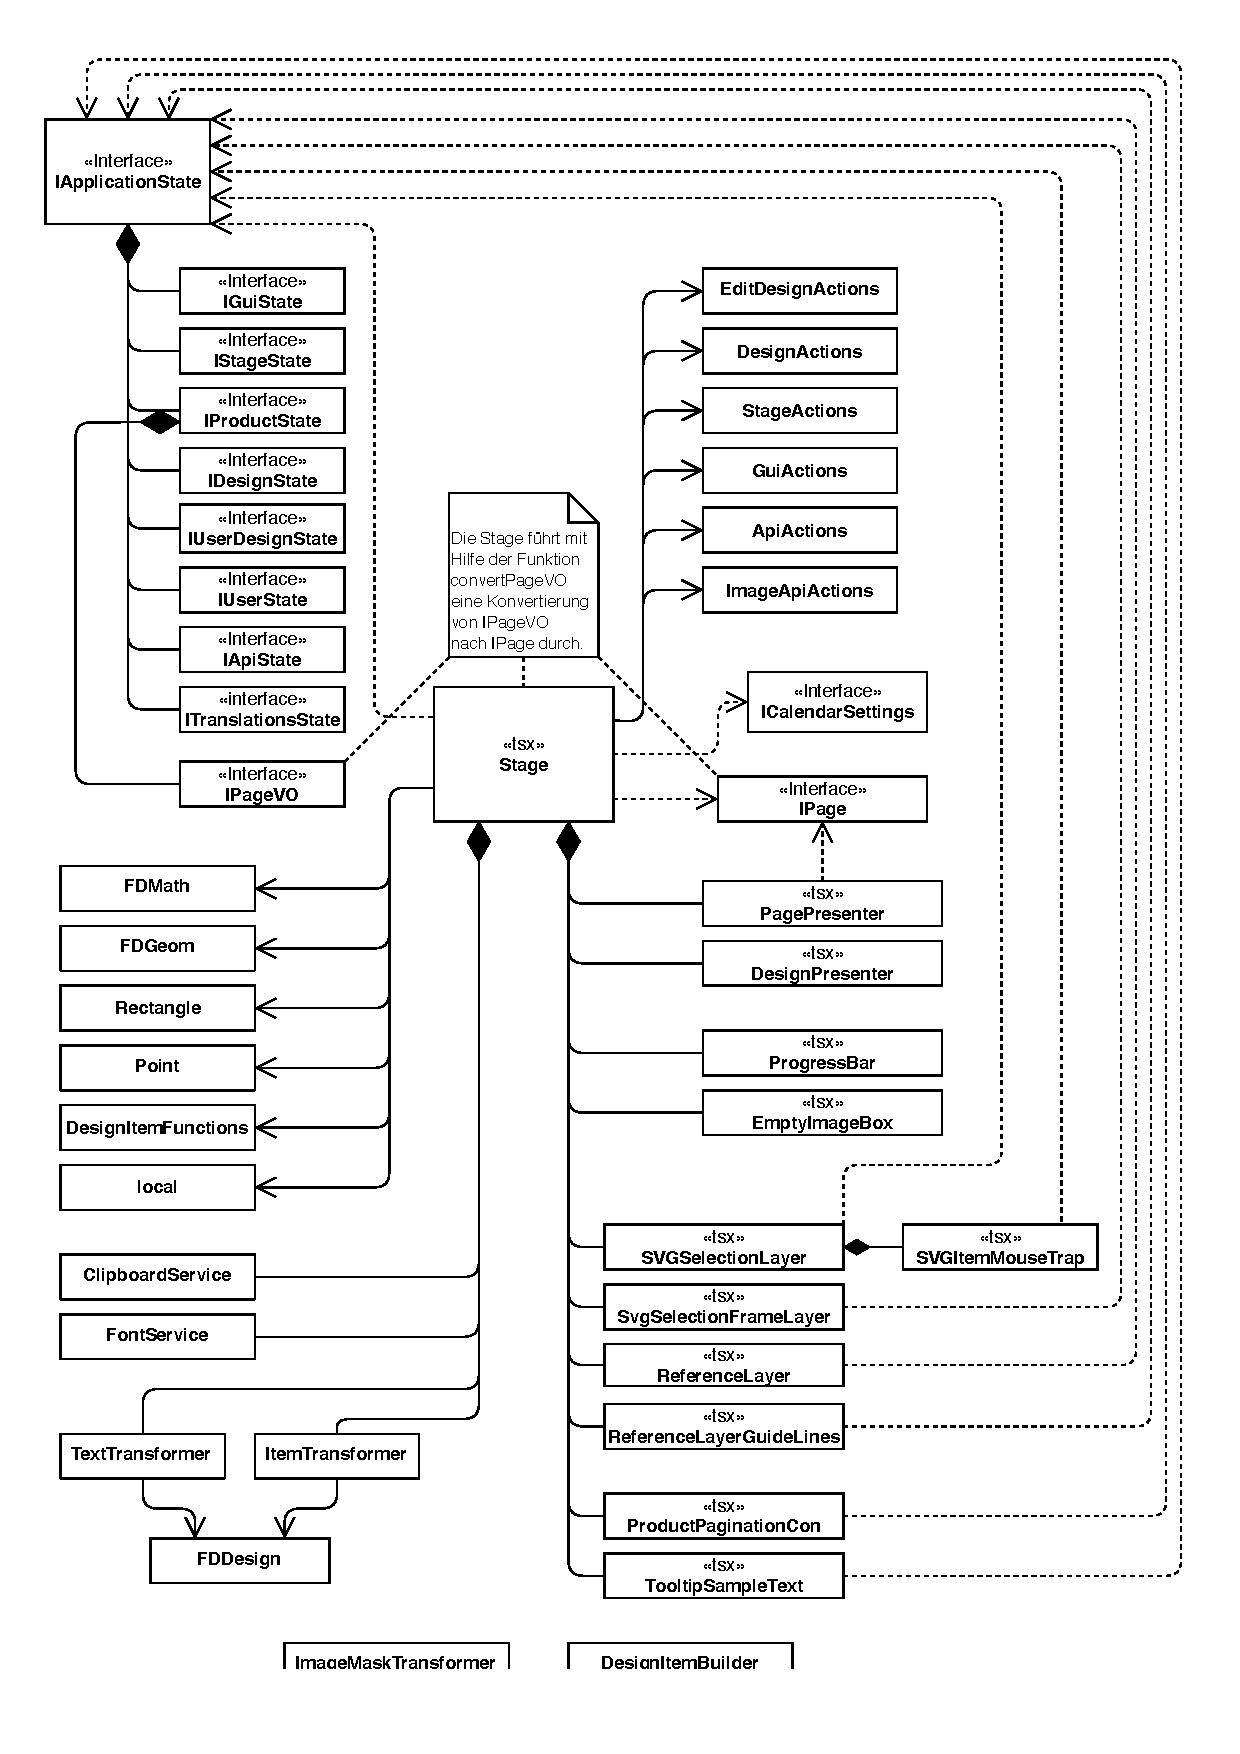
\includegraphics[width=1\textwidth]{diagrams/Ist-Architektur/Designbearbeiten.pdf}
    \caption{Zusammenhänge der Komponente zum Bearbeiten eines Designs}
    \label{fig:Designbearbeiten}
\end{figure}
Die Darstellung der Stage basiert auf Teilen des \emph{Redux-State} der durch die Schnittstelle \lstinline|IApplicationState| beschrieben wird. Dieser fasst weitere Zustände zusammen die jeweils als Schnittstellen beschrieben sind. Durch die Schnittstelle \lstinline|IGuiState| wird der Zustand der grafischen Oberfläche des FreeDesign-Editors beschrieben. Beischspiele hierfür sind 
ob und welcher modale Dialog dargestellt wird oder wie im aktuellen Zustand das Menü für ein Designobjekt aufgebaut ist.
Vom Zustand der grafischen Oberfläche entkoppelt, wird durch die Schnittstellen \lstinline|IStageState| der Zustand der Stage beschrieben. Beispielsweise wird durch sie beschrieben, mit welchem Skalierungsfaktor und durch welchen Rotation die Produktseite auf der Stage dargestellt wird. Die Schnittstelle \lstinline|IProductState| beschreibt das Produkt welches vom Nutzer im FreeDesign-Editor bearbeitet wird. 
Durch die Schnittstelle \lstinline|IDesignState| wird das Design, welches vom Nutzer gestaltet wird, beschrieben. Hierfür verwalte die Schnittstelle ein zweidimensionales Array, welches in der der ersten Dimension eine Listen  der einzelnen Produktseiten abbildet und in der zweiten Dimension eine Liste der Designobjekte der Einzelseiten. Für das Verwalten von Metadaten eines Kundendesigns, wie der Designname unter dem ein Design gespeichert wurde oder der Zeitstempel, wann ein Design erstellt, wird durch die Schnittstelle \lstinline|IUserDesignState| beschrieben. 
Der \emph{Redux-State} besitzt auch eine Zustandsbeschreibung für Daten des Nutzers, welche durch die Schnittstelle \lstinline|IUserState| beschrieben wird. Die bereits genannten Zustände, \lstinline|IProductState|, \lstinline|IDesignState|, \lstinline|IUserDesignState| und \lstinline|IUserState| werden von Werte belegt, die durch API bereitgestellt werden. Allerdings besitz der \emph{Redux-State} ein weiteres Unterobjekt, welches durch die Schnittstelle  \lstinline|IApiState| beschrieben wird und ebenfalls durch Daten der API beschrieben wird. Hierzu zählt eine Liste von Schriftarten, die innerhalb eines Designs genutzt werden können, sowie eine Liste der Bilder, die ein Kunde in seinem Design nutzt.  
Das Objekt welches durch die Schnittstellen \lstinline|ITranslationsState| beschrieben wird, enthält lediglich eine Liste von Texten, die durch den FreeDesign-Editor genutzt werden und ebenfalls durch API bereitgestellt werden. 

Die Stage greift auf den \emph{Redux-State} zu und stellt durch die Nutzung der React-Komponenten \lstinline|PagePresenter| und \lstinline|DesignPresenter| dass im State gespeicherte Produkt und Design dar.

Weiterhin nutzt die Stage die Container-Komponente \lstinline|SVGSelectionLayer|, welche wiederrum die Container-Komponente \lstinline|SVGItemsMouseTrap| nutzt. Beide Komponente ermöglichen das Auswählen von Designobjekten und stellen diese Auswahl durch eine Umrahmung der Objekte dar. Neben der Darstellung eine Auswahlrahmens stellen die Komponenten Schaltflächen bereit, über welche die \emph{Redux-Action} \lstinline|GuiActions.setEditorMode(mode: EditorMode)| augerufen wird. Der Action wird ein Modus übergeben welcher im \emph{Redux-State} unter \lstinline|IGuiState.editorMode| gesetzt wird. Der so übergeben Modus bestimmt die Transformationsart mit der eine Objekt bearbeitet werden soll. So wird Beispielsweise definiert, ob ein Objekt verschoben, rotiert oder skaliert werden soll. Wenn der Zustand \lstinline|editorMode|  durch einen solchen Wert belegt ist, wird von der Stage Maus- und Tastatureingabe verarbeitet. Auf Basis der Eingaben werde mit Hilfe der Klasse \lstinline|ItemTransformer|, bzw. bei Texteingaben der Klasse \lstinline|TextTransformer|, neue Designobjekte erzeugt.  
Die Stage übergebt die so neu berechneten Designobjekte der \emph{Redux-Action} \lstinline|EditDesignActions.updateDesignItems()| wodurch das Design im \emph{Redux-State} wird.

Für Bildobjekt besteht außerdem die Möglichkeit über den modalen Dialog den Bildausschnitt zu bearbeiten. Für die Steuerung des Dialogs und die Verarbeitung von Mauseingaben ist die Container-Komponente \lstinline|ImageMaskEditor.tsx| zuständig. Ein neues Bildobjekt wird mit Hilfe der Klasse \lstinline|ImageMaskTransformer| berechnet. 

Die Container-Komponente \lstinline|DesignItemMenu.tsx| stellt ein Menü bereit welches in Abhängigkeit zu den Ausgewählten aufgebaut ist und weitere Optionen zur Änderungen der Designobjekte biete. Beispiele hierfür sind das Ändern von Farben, Schriftarten oder Linienstärken. Für jeden Änderung wird ebenefalls die \emph{Redux-Actions}  aus dem Modul \lstinline|EditDesignActions.ts| augerufen, die das Design im \emph{Redux-State} aktualisieren.

Über die Container-Komponente \lstinline|ToolBox.tsx| können dem Design neue Elemente hinzugefügt werden.  Was durch den Aufruf der \emph{Redux-Action}  \lstinline|EditDesignActions.addDesignItems()| erfolgt.

Für die Bereitstellung der Funktionalität zum widerrufen bzw. widerherzustellen einer Eingabe, enthält die Schnittstelle \lstinline|IStageState| das Attribut \lstinline|pageForHistory|. 
Die \emph{Redux-Actions} zur Steuerung der Historie sind ebenfalls im Modul \lstinline|EditDesignActions.ts| enthalten.

Durch die Container-Komponente \lstinline|SVGSelectionFrameLayer| wird die Funktionalität umgesetzt, mit der Maus einen Auswahlrahmen zur Auswahl mehrerer Designobjekte zu erzeugen. 

Für das Bearbeiten einens Designs werden die grafischen Hilfsmittel Lineal, Gitter und Hilfslinien bereitgestellt.
Diese werden durch die Container-Komponenten \lstinline|ReferenceLayer| \lstinline|ReferenceLayerGuideLines| erzeugt. 

Wird ein Produkt mit mehr als einer Seite bearbeitet wird dem Nutzer mit Hilfe der Container-Komponenten \lstinline|ProductPaginationCon| eine Paginierung der Seiten dargestellt. Diese stellt eine Vorschau der einzelnen Designseiten dar, weshalb sie auf die Komponenten \lstinline|PagePresenter| und \lstinline|DesignPresenter| zugreift.


% TODO: npx depcruise -- config W1_dependency - cruiser - konfiguration . json -T dot
% src / containers / stage | dot -T svg > Designeditieren .svg


% TODO: npx depcruise -- config W1_dependency - cruiser - konfiguration . json -T dot
% src / designToSvgCLI | dot -T svg > SVG - Konvertierung .svg

Die dritte Hauptkomponente des FreeDesign-Editors ist das bearbeiten des Designs. Hierfür stellt der Editor Eingabekomponenten zur Verfügung, welche Änderungen der Designstruktur im \emph{Redux-State} bewirken. Auf diese Änderungen reagiert die Designdarstellung und löst eine Aktualisierung aus, wodurch keine Abhängigkeiten zwischen der Darstellung des Designs und der Bearbeitung des Designs bestehen. Beide Komponenten greifen lediglich auf die selbe Designstruktur zu.  
Die \emph{Container}-Komponente \emph{Stage.tsx} verbindet alle Komponenten, die für die Bearbeitung des Designs Notwendig sind. Hierzu gehören grafisch Komponente zur Darstellung von Auswahlrahmen, eine Texteingabe sowie Hilfswerkzeugen, wie einem Lineal oder einem Gitter. 
Desweiteren ist sie mit dem \emph{Redux-Store} verbunden und ruft sie verschieden \emph{Redux-Actions}. 

Im allgemeinen ist der Quelltext und die Abhängigkeiten für die Designbearbeitung sehr komplex und ungenügend strukturiert. 
Ein Darstellung der gesamten Abhängigkeiten ist im Anhang unter \emph{D2\_Designbearbeitung.html} enthalten.
Das bearbeiten eines Designs ist die Kernfunktionalität des FreeDesign-Editor und sollte von einer Soll-Architektur aus der restlichen Anwendung als entkoppelte Komponente extrahiert werden. 



Folgende Bausteine wurden identifiziert, für die Designbearbeitung notwendig sind.
\begin{multicols}{2}    
    \begin{enumerate}
\item{API-Kommunikation} 
\item{Bildverarbeitung}  
\item{Cache} 
\item{Cookie-Verarbeitung}  
\item{Design-Parser} 	
\item{Designbearbeitung} 
\item{Designdarstellung}  
\item{Designobjekt-Transformation}
\item{Designobjekterzeugung} 
\item{Designstruktur} 
\item{Farbstruktur} 
\item{Grafische-Oberfläche} 
\item{Kalendariumerzeuger} 
\item{Mathematik}  
\item{Produktdarstellung} 
\item{Produktstruktur} 
\item{SVG-Parser} 
\item{Textschlüsselsammlung} 
\item{URL-Verarbeitung} 
\item{Vorlagekonverter} 
\item{XML-Parser}	
\end{enumerate} 
\end{multicols}
